%%%%%%%%%%%%%%%
%%%%%%%%%%%%%%%
\begin{frame}
    \shiftedframetitle{2. Theory}
    \vspace{2cm}
\centering
\includegraphics[scale=1]{Resources/Images/imagesThesis/arrowpach.png}
%{\Huge\textbf{Shallow Water Equations}}
\end{frame}


%%%%%%%%%%%%%%%%%%%%
%%%%%%%%%%%%%%%%%%%%

\begin{frame}
    \shiftedframetitle{2. Theory}
%\vspace{-1.5cm}
\begin{minipage}{0.35\textwidth}
%\vspace{-3mm}
\begin{itemize}
\item<1->[]
\begin{align*}
\frac{\partial u}{\partial x} + \frac{\partial v}{\partial y} + \frac{\partial w}{\partial z} &= 0
\end{align*}
\item<1->[]
\begin{align*}
\frac{\partial u}{\partial t} + u\frac{\partial u}{\partial x} + v\frac{\partial u}{\partial y} + w\frac{\partial u}{\partial z} &= - \frac{\partial p}{\partial x}
\end{align*}
\item<1->[]
\begin{align*}
\frac{\partial v}{\partial t} + u\frac{\partial v}{\partial x} + v\frac{\partial v}{\partial y} + w\frac{\partial v}{\partial z}&= - \frac{\partial p}{\partial y}
\end{align*}
\item<1->[]
\begin{align*}
\frac{\partial w}{\partial t} + u\frac{\partial w}{\partial x} + v\frac{\partial w}{\partial y} + w\frac{\partial w}{\partial z} &= - \frac{\partial p}{\partial z} + g \end{align*}
\end{itemize}
\end{minipage}
%\hspace{1.5cm}
%\begin{minipage}{0.5\textwidth}
%\vspace{3cm}
%\includegraphics[width=\textwidth]{./Resources/Images/imagesThesis/floor.png}
%\end{minipage}
\end{frame}
\clearpage

%%%%%%%%%%%%%%%%%%%%
%%%%%%%%%%%%%%%%%%%%

\begin{frame}
    \shiftedframetitle{2. Theory}
%\vspace{-0.5cm}
\begin{minipage}{0.3\textwidth}
\begin{itemize}
\item<1->[]
\begin{align*}
\color{TUMOrange}\underbrace{\color{black}\frac{\partial u}{\partial x} + \frac{\partial v}{\partial y}}_{\approx \frac{2U}{L}} \color{black} + \color{TUMOrange}\underbrace{\color{black}\frac{\partial w}{\partial z}}_{\myTUMorange{\approx \frac{W}{H}}} &= 0 \quad \myTUMorange{\rightarrow} \quad \color{TUMOrange}\underbrace{W \approx -2U \frac{H}{L}}_{\approx\ 0 \ if\  L>>H} \qquad \qquad \quad
\end{align*}
\item<2->[]
\begin{align*}
\frac{\partial u}{\partial t} + u\frac{\partial u}{\partial x} + v\frac{\partial u}{\partial y} + w\frac{\partial u}{\partial z} &= - \frac{\partial p}{\partial x}\\[0.5cm]
\frac{\partial v}{\partial t} + u\frac{\partial v}{\partial x} + v\frac{\partial v}{\partial y} + w\frac{\partial v}{\partial z}&= - \frac{\partial p}{\partial y}\\[0.5cm]
\color{TUMDarkBlue}\underbrace{\color{black}\frac{\partial w}{\partial t} + u\frac{\partial w}{\partial x} + v\frac{\partial w}{\partial y} + w\frac{\partial w}{\partial z}}_{\myTUMdarkblue{0}}  \color{black} &= - \frac{\partial p}{\partial z} + g\\ \quad \myTUMdarkblue{\rightarrow} \quad \myTUMdarkblue{0} &\myTUMdarkblue{= - \frac{\partial p}{\partial z} + g}
\end{align*}
\end{itemize}
\end{minipage}
\hspace{-2.5cm}
\begin{minipage}{0.15\textwidth}
\begin{itemize}
\item<3->[]
%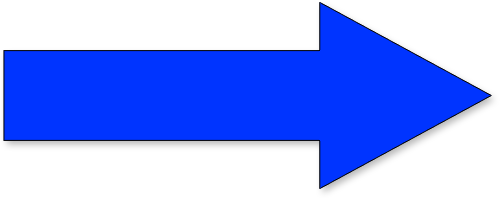
\includegraphics[width=1\textwidth]{Resources/Images/download.png}\\[2cm]
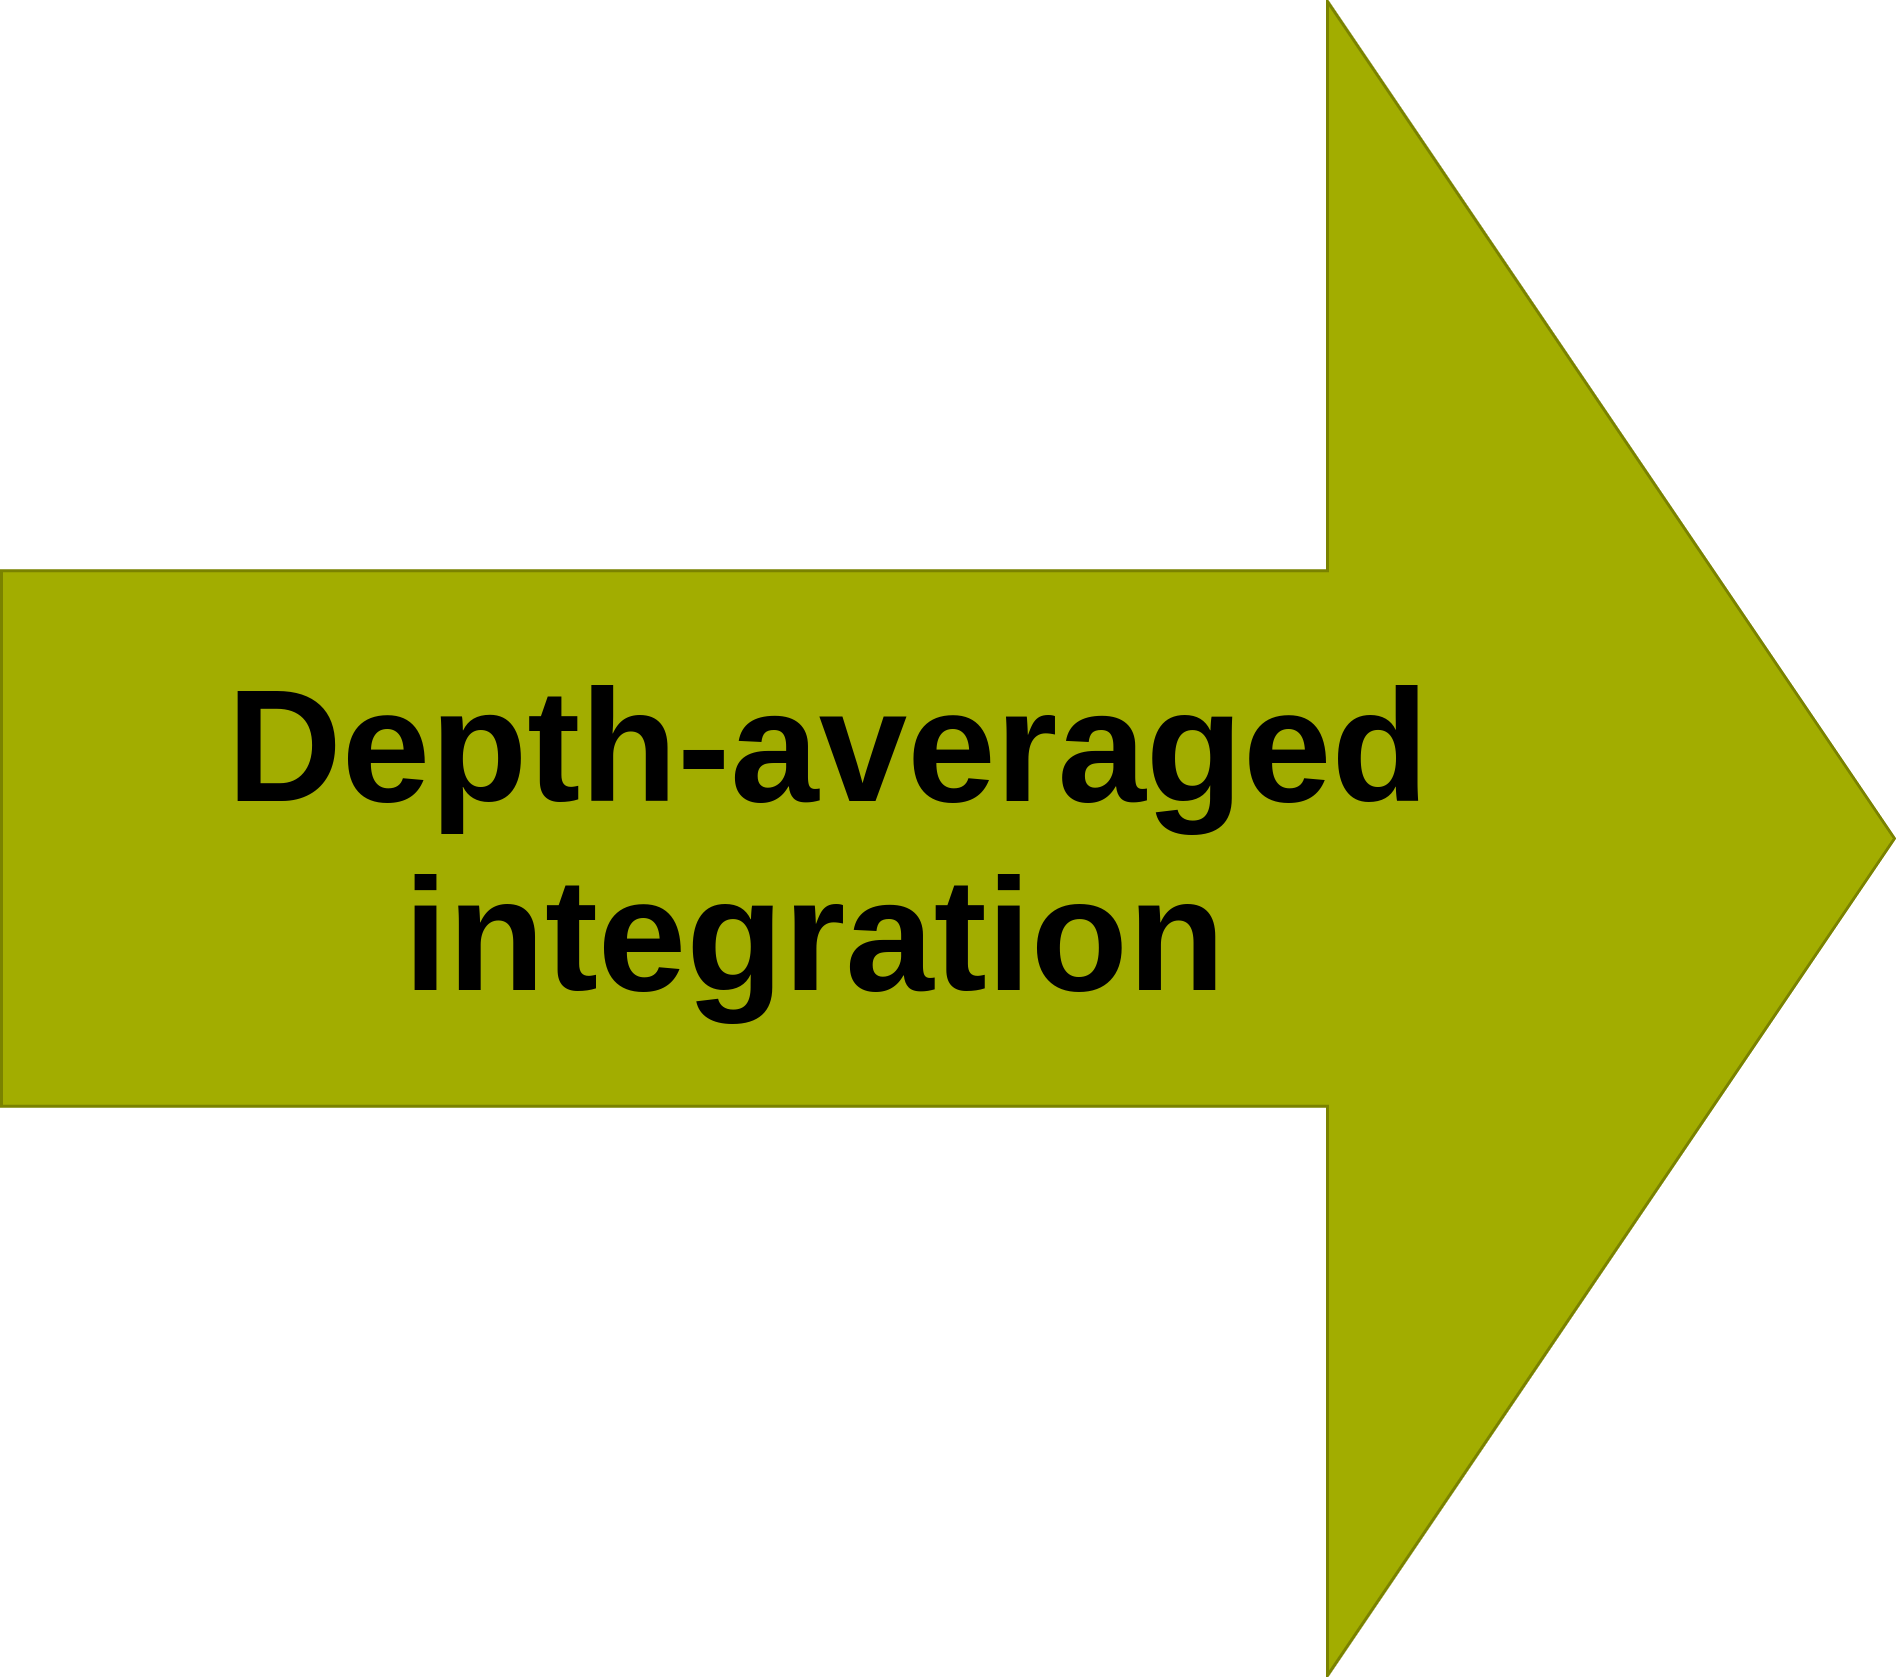
\includegraphics[width=1.2\textwidth]{Resources/Images/arrow3.png}\\
\end{itemize}           
\end{minipage}
\hspace{1.5cm}
\vspace{-1cm}
\begin{minipage}{0.4\textwidth}
\begin{itemize}
\item<3->[]
% \hspace{1.5cm}
%\begin{minipage}{0.5\textwidth}
%\vspace{3cm}
\centering
%\hspace*{0pt}\hfill
\includegraphics[width=0.8\textwidth]{./Resources/Images/imagesThesis/diag.png}
%\end{minipage}
\item<3->[]
\begin{tcolorbox}[title=SWE model, colback=white] 
\begin{align*}
\myTUMgreen{\frac{\partial h}{\partial t}} + \frac{\partial \myTUMgreen{h}u}{\partial x} + \frac{\partial \myTUMgreen{h}v}{\partial y} &= 0\\[0.5cm]
\frac{\partial \myTUMgreen{hu}}{\partial t} + \frac{\partial}{\partial x}(\myTUMgreen{hu^2} + \myTUMdarkblue{\frac{1}{2} g h^2}) + \frac{\partial \myTUMgreen{huv}}{\partial y} &= \myTUMdarkblue{- gh\frac{\partial b}{\partial x}} \\[0.5cm]
\frac{\partial \myTUMgreen{hv}}{\partial t} + \frac{\partial \myTUMgreen{huv}}{\partial x} + \frac{\partial}{\partial y}(\myTUMgreen{hv^2} + \myTUMdarkblue{\frac{1}{2} g h^2})&= \myTUMdarkblue{- gh\frac{\partial b}{\partial y} }
\end{align*}
\end{tcolorbox}
\end{itemize}
\end{minipage}
\end{frame}
\clearpage


%%%%%%%%%%%%%%%%%%%%
%%%%%%%%%%%%%%%%%%%
\begin{frame}
    \shiftedframetitle{2. Theory }
{\large Navier-Stokes $\rightarrow$ \textbf{free-surface problems}}
\begin{itemize}
\item<2-> \textbf{Multi-phase solver} $\rightarrow$ Volume-of-Fluid Method (VOF): Fluid A and Fluid B:
\item<3-> \textbf{Volume indicator function} $\rightarrow \alpha$ 
\begin{align*}
\alpha(\mathbf{x},t)=\begin{cases}
    1, & \text{water}\\
    0, & \text{air}\\
    0<\alpha<1, & \text{surface}
  \end{cases}
\end{align*}
\item<4-> \textbf{$\alpha$ transport equation:}
\begin{align*}
\frac{\partial \alpha}{\partial t} + \nabla \cdot (\alpha \mathbf{u}) + \nabla \cdot (\alpha (1 - \alpha)\mathbf{u_r}) = 0\\
\rho(\alpha) = \alpha\rho_A + (1-\alpha)\rho_B
\end{align*}
\end{itemize}


\end{frame}
\clearpage

%%%%%%%%%%%%%%%%%%%%
%%%%%%%%%%%%%%%%%%%
\begin{frame}
    \shiftedframetitle{2. Theory}

%The SWE:
%\begin{itemize}
%\setlength\itemsep{1.8em}
%\item<1-> \textbf{simplify} \textit{$3D$} Navier-Stokes \textit{to} a \textit{$2D$} system of equations
%\item<2-> \textit{\textbf{neglect} vertical velocity}:  $ W \ll U,V $, horizontal distances $L$ $\gg$ vertical distance $H$
%\item<3-> represent a \textbf{hyperbolic PDE} system $\rightarrow$ Riemann Problem
%\item<4-> \textbf{Applications}: 
%\begin{itemize}
%\addtolength{\itemindent}{1cm}
%\item Free-surface flows around structures, 
%\item Tsunamis prediction,
%\item Atmospheric flows, \dots
%\end{itemize}
%\item<5->[]
%\hspace{5cm}
\vspace{2.5cm}
\centering
\includegraphics[scale=1]{Resources/Images/imagesThesis/message2.png}
%\begin{minipage}{0.5\textwidth}
%\begin{tcolorbox}[colback=white] 
%NS and SWE reach a solution for free-surface problems \\[2cm]\centering $\downarrow$\\[1cm] \textbf{\textit{compatibility between the respective solution methods}}
%\end{tcolorbox}
%\end{minipage}
%\end{itemize}
\end{frame}
\clearpage

%%%%%%%%%%%%%%%
%%%%%%%%%%%%%%%
\begin{frame}
    \shiftedframetitle{2. Theory}
    \vspace{4cm}
\centering
{\Huge\textbf{Flow Characterization}}
\end{frame}


%%%%%%%%%%%%%%%%%
%%%%%%%%%%%%%%%%%
\begin{frame}
    \shiftedframetitle{2. Theory}
\begin{minipage}{0.45\textwidth}
\begin{itemize}
\vspace{1cm}
\item<1->[] 
\centering
{\LARGE \textbf{Subcritical flow}}\\[0.15cm]
\hspace{0.2cm}
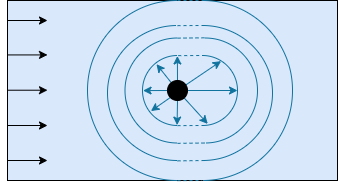
\includegraphics[width=1\textwidth]{Resources/Images/subcritical.png}
\end{itemize}
\end{minipage}
\hspace{1cm}
\begin{minipage}{0.45\textwidth}
\centering
\begin{itemize}
\vspace{1cm}
\item<2->[] 
\centering
{\LARGE \textbf{Supercritical flow}}\\[0.15cm]
\hspace{0.25cm}
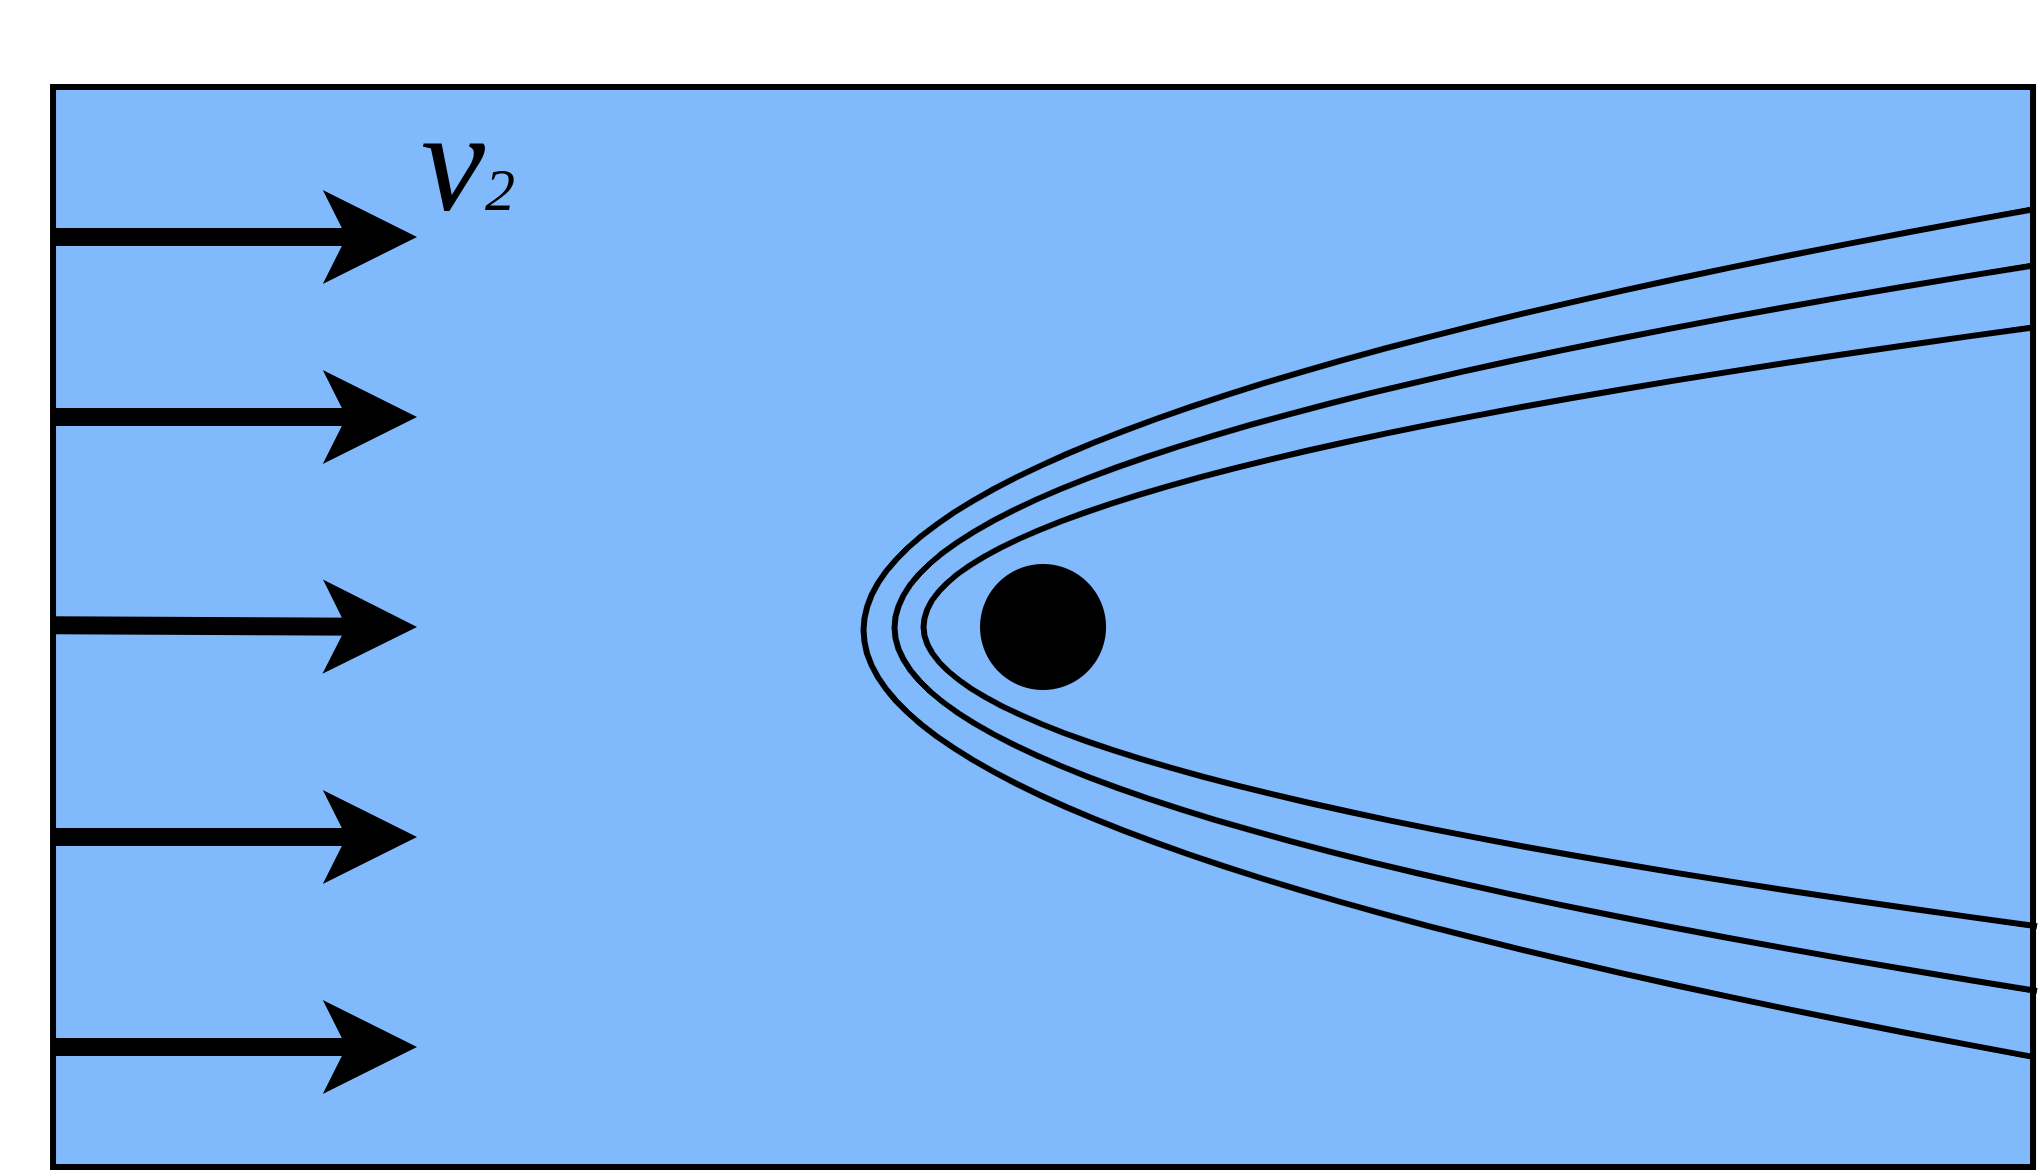
\includegraphics[width=1\textwidth]{Resources/Images/supercritical.png}
\end{itemize}
\end{minipage}
\end{frame}

\clearpage


